\documentclass[11pt]{standalone}

\usepackage{fontspec}
\usepackage{unicode-math}

\setmainfont{TeX Gyre Pagella}
\setsansfont{Linux Biolinum O}
\setmathfont{TeX Gyre Schola Math}

\usepackage{ifthen}
\usepackage{amsmath}

\usepackage[d]{esvect}
\usepackage[svgnames]{xcolor}
\usepackage{tikz}
\usetikzlibrary{shapes.misc}
\usetikzlibrary{arrows,arrows.meta}
\usetikzlibrary{calc,intersections, patterns, math}

\definecolor{pfeil}{RGB}{168,167,167}
\definecolor{salmon}{RGB}{250,128,114}
\definecolor{petrol}{RGB}{0, 118, 136}
\definecolor{darkgoldenrod}{RGB}{184, 134, 11}
\colorlet{petrol-lighter}{petrol!40}
\colorlet{darkgoldenrod-lighter}{darkgoldenrod!40}

\tikzset{>={Stealth[scale=1.25]}}

\begin{document}

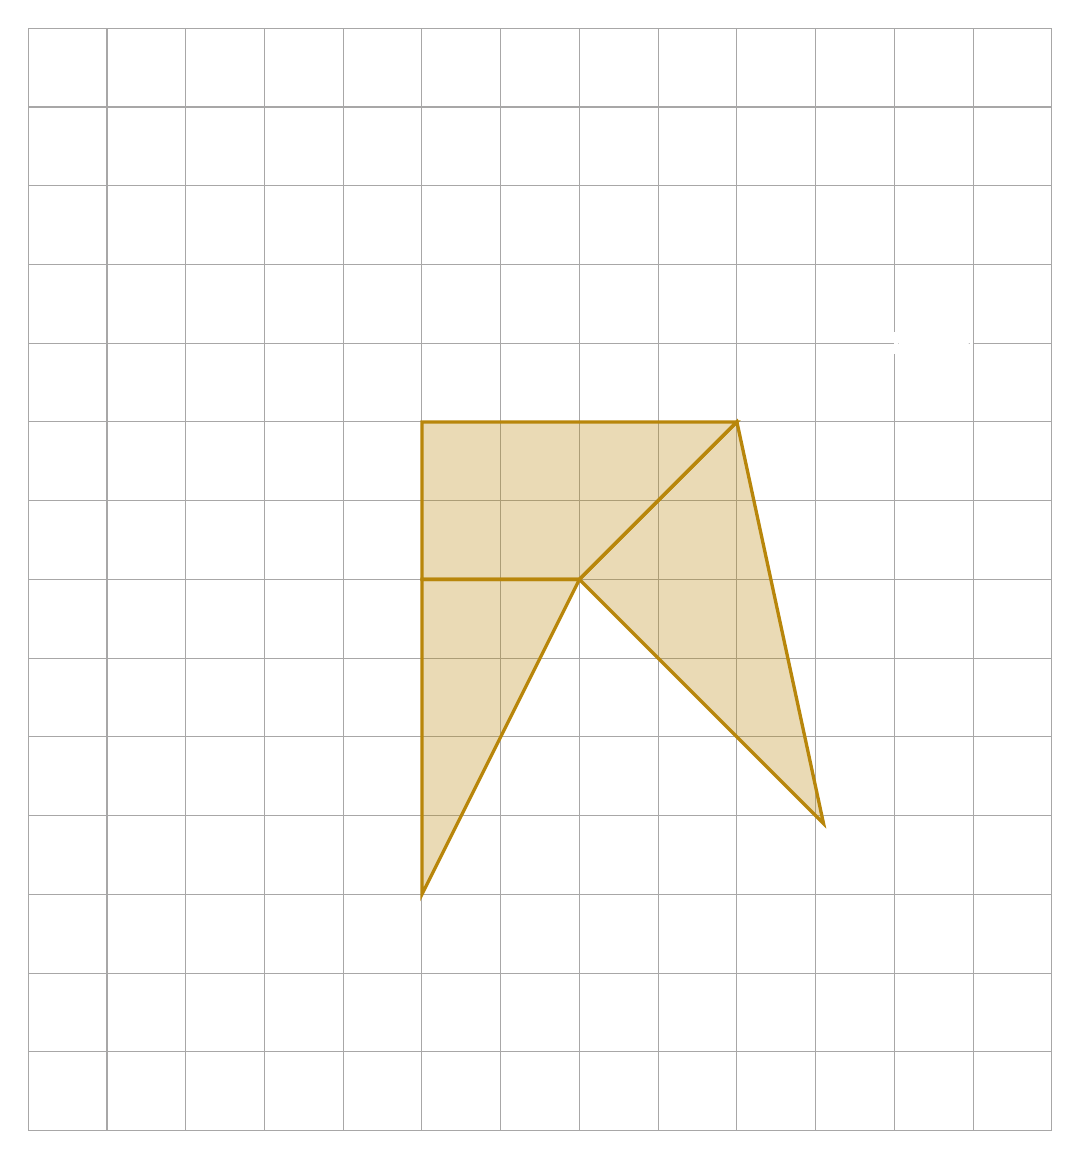
\begin{tikzpicture}[pfeil, very thick]
			
	\draw[thin, step=1] (0,0) grid (13,14);

	\draw[|<->|, white] (11,10) -- node[above] {$1\,\text{LE}$} (12,10);

	\draw[darkgoldenrod, fill, fill opacity = 0.3] (5,7) -- (7,7) -- (9,9) -- (5,9) -- cycle;
	\draw[darkgoldenrod, fill, fill opacity = 0.3] (5,7) -- (7,7) -- (5,3) -- cycle;
	\draw[darkgoldenrod, fill, fill opacity = 0.3] (7,7) -- (10.1,3.9) -- (9,9) -- cycle;
\end{tikzpicture}			

\end{document}
